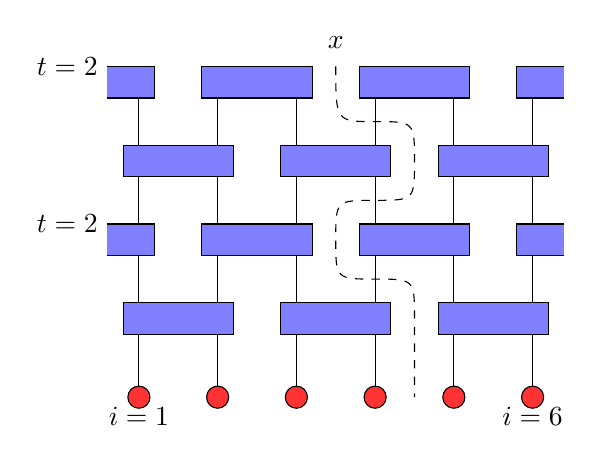
\begin{tikzpicture}[scale = 1]
\draw (0,0) node[below]{$i=1$} -- (0,4);
\filldraw[color=black, fill=red!80] (0,0) circle (4pt) node[anchor=west] { };
\draw (1,0) -- (1,4);
\filldraw[color=black, fill=red!80] (1,0) circle (4pt) node[anchor=west] { };
\draw (2,0) -- (2,4);
\filldraw[color=black, fill=red!80] (2,0) circle (4pt) node[anchor=west] { };
\draw (3,0) -- (3,4);
\filldraw[color=black, fill=red!80] (3,0) circle (4pt) node[anchor=west] { };
\draw (4,0) -- (4,4);
\filldraw[color=black, fill=red!80] (4,0) circle (4pt) node[anchor=west] { };
\draw (5,0) node[below]{$i=6$} -- (5,4);
\filldraw[color=black, fill=red!80] (5,0) circle (4pt) node[anchor=west] { };

\foreach \x/\y in {0/1, 2/1, 4/1, 1/2, 3/2, 0/3, 2/3, 4/3, 1/4, 3/4} 
\filldraw[color=black, fill=blue!50] (\x-.2,\y-.2) rectangle (\x+1.2,\y+.2);

\draw[fill=blue!50] (-.4,1.8) -- (.2,1.8) -- (.2,2.2) -- (-.4,2.2)
								node[left] {$t=2$};
\draw[fill=blue!50] (-.4,3.8) -- (.2,3.8) -- (.2,4.2) -- (-.4,4.2)
								node[left] {$t=2$};
\draw[fill=blue!50] (5.4,4.2) -- (4.8,4.2) -- (4.8,3.8) -- (5.4,3.8);
\draw[fill=blue!50] (5.4,2.2) -- (4.8,2.2) -- (4.8,1.8) -- (5.4,1.8);

\draw (2.5,4.5) node{$x$};
\draw[dashed] (2.5,4.2) .. controls (2.5,3.5) .. (3,3.5) 
                        .. controls (3.5,3.5) .. (3.5,3) 
                        .. controls (3.5,2.5) .. (3,2.5) 
                        .. controls (2.5,2.5) .. (2.5,2) 
                        .. controls (2.5,1.5) .. (3,1.5) 
                        .. controls (3.5,1.5) .. (3.5,1) 
                        .. controls (3.5,0.5) .. (3.5,0.5) 
                        .. controls (3.5,0.0) .. (3.5,0);
\end{tikzpicture}